\documentclass[notheorems,serif,table,compress]{beamer}  %dvipdfm选项是关键,否则编译统统通不过
%%------------------------常用宏包------------------------
%%注意, beamer 会默认使用下列宏包: amsthm, graphicx, hyperref, color, xcolor, 等等
\usepackage{fontspec,xunicode,xltxtra}  % for XeTeX
\usepackage{verbatim}
%\usepackage{mathabx}
\usepackage{latexsym}
\usepackage{amsfonts,amssymb}
\usepackage{styles/iplouclistings}
\usepackage{fancybox}
\usepackage{colortbl}
\usepackage{tcolorbox}
%\usepackage[T1]{fontenc}
%\usepackage{bookman}
\usepackage{subfigure}
\usepackage{hyperref}
\usepackage{listings}
\usepackage{animate}
\usepackage[absolute,overlay]{textpos}
\usepackage{graphicx}
\usepackage{tikz}
\usepackage[americaninductors,europeanresistors]{circuitikz}
\usepackage{tikz}
\usepackage{fancybox}     %% 定义zhushadow时用到
\usepackage{pifont} %ding用到
\newsavebox{\mysaveboxOne}  %%为了在only中使用lstlisting
\newsavebox{\mysaveboxTwo}
\newsavebox{\mysaveboxThree}
\newsavebox{\mysaveboxFour}
\newsavebox{\mysaveboxFive}
\newsavebox{\mysaveboxSix}
\newsavebox{\mysaveboxSeven}
\newcommand\zhushadow[2][purple]{\hskip5pt\shadowbox{\color{#1}\small\kai #2\vspace{3mm}}}

%%------------------------ThemeColorFont------------------------
%% Presentation Themes
% \usetheme[<options>]{<name list>}
%\usetheme{Madrid}
\usetheme{Berkeley}
%% Inner Themes双精度计算
% \useinnertheme[<options>]{<name>}
%% Outer Themes
% \useoutertheme[<options>]{<name>}
%\useoutertheme{miniframes} 
%% Color Themes 
%\usecolortheme[<options>]{<name list>}
%% Font Themes
\usefonttheme{serif}
\setbeamertemplate{background canvas}[vertical shading][bottom=white,top=structure.fg!7] %%背景色, 上25%的蓝, 过渡到下白.
\setbeamertemplate{theorems}[numbered]
\setbeamertemplate{navigation symbols}{}   %% 去掉页面下方默认的导航条.
\usepackage{styles/zhfontcfg}
%\setsansfont[Mapping=tex-text]{文泉驿正黑}  %% 需要fontspec宏包
     %如果装了Adobe Acrobat,可在font.conf中配置Adobe字体的路径以使用其中文字体
     %也可直接使用系统中的中文字体如SimSun,SimHei,微软雅黑 等
     %原来beamer用的字体是sans family;注意Mapping的大小写,不能写错
     %设置字体时也可以直接用字体名,以下三种方式等同:
     %\setromanfont[BoldFont={黑体}]{宋体}
     %\setromanfont[BoldFont={SimHei}]{SimSun}
     %\setromanfont[BoldFont={"[simhei.ttf]"}]{"[simsun.ttc]"}
%%------------------------MISC------------------------
\graphicspath{{figures/}}         %% 图片路径. 本文的图片都放在这个文件夹里了.
%%------------------------listing------------------------
%\lstset{language=[LaTeX]TeX,Python}
%%------------------------正文------------------------
\begin{document}
\XeTeXlinebreaklocale "zh"         % 表示用中文的断行
\XeTeXlinebreakskip = 0pt plus 1pt % 多一点调整的空间
%%----------------------------------------------------------
%% This is only inserted into the PDF information catalog. Can be left
%% out.
%%%
%% Delete this, if you do not want the table of contents to pop up at
%% the beginning of each subsection:
%\AtBeginSection[]{                              % 在每个Section前都会加入的Frame
%  \frame<handout:0>{
%    \frametitle{Contents}\small
%    \tableofcontents[current,currentsubsection]
%  }
%}
%
%\AtBeginSubsection[]                            % 在每个子段落之前
%{
%  \frame<handout:0>                             % handout:0 表示只在手稿中出现
%  {
%    \frametitle{Contents}\small
%    \tableofcontents[current,currentsubsection] % 显示在目录中加亮的当前章节
%  }
%}

\setbeamertemplate{caption}{\raggedright\insertcaption\par}

%%----------------------------------------------------------
\logo{
\includegraphics[scale=0.13]{ouclogo.png}}
\title{Image Interpolation}
%\subtitle{Bottom-Up Saliency Detection Model Based on Human Visual Sensitivity and Amplitude Spectrum}
\subtitle{图像内插}
\author[]{\textcolor{black}{DingHao}}
\institute[CVBIOUC]
{
\small\textcolor{violet}{CVBIOUC\\
%Ocean University of China\\
\url{http://vision.ouc.edu.cn/~zhenghaiyong}}
}
%\date[]{}
%\titlegraphic{
%\includegraphics[height=1.0cm]{ouc-logo.jpg}}
\frame{ \titlepage }

%%----------------------------------------------------------
%\section*{Contents}

\frame{\frametitle{Contents}\tableofcontents}


%%----------------------------------------------------------
\def\hilite<#1>{\temporal<#1>{\color{blue!15}}{\color{black}}{\color{black}}}
\newcommand{\shadow}[2][purple]{\hskip5pt\shadowbox{\color{#1}\small \kai #2\vspace{3mm}}}
\newcommand{\colorrbox}[2][purple]{\doublebox{\color{#1}\small \kai#2}}

%============================================================================

\section{Introduction}

\subsection{Brief Introduction}
\begin{frame}[fragile]
\frametitle{Brief Introduction}
    Image interpolation is a method of constructing new data points within the range of a discrete set of known data points.

    Functions:	
	\begin{itemize}
	\item Scaling
	\item Rotate
	\item Geometric Correction
    	\end{itemize}
\end{frame}

\subsection{Relarge Images}
\begin{frame}
\frametitle{Relarge Images}
    The purpose of enlarging image (upsamplin / interpolating) is to enlarge the original image so that it can be displayed on a higher -resolution display device.
	\begin{figure}
        \begin{minipage}[t]{0.4\linewidth}
        \centering
        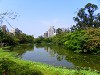
\includegraphics[width=0.3\linewidth]{template.png} 
        \end{minipage}
        \begin{minipage}[t]{0.4\linewidth}
        \centering
        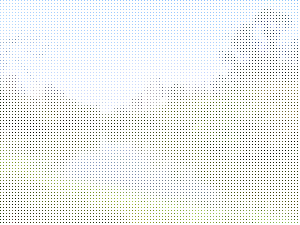
\includegraphics[width=1\linewidth]{template1.png} 
        \end{minipage}
   	\end{figure}
%图像放大几乎都是采用内插值方法,即在原有图像像素的基础上在像素点之间采用合适的插值算法插入新的元素。
\end{frame}
 
\subsection{classification}

\begin{frame}
\frametitle{Classification}
	\begin{cases}
	$Traditional algorithm$	
		\begin{cases}
		$Nearest neighbor interpolation$\\
		$Bilinear interpolation$\\
		$Bicubic interpolation$
		\end{cases}\\
	$Interpolation based on edge$
		\begin{cases}
		$Low-resolution$\\
		$High-resolution$
		\end{cases}\\
	$Interpolation based on area$\\
	$Other methods$
	\end{cases}
\end{frame}


\section{Nearest neighbor interpolation}

\subsection*{Theory}
\begin{frame}
\frametitle{Nearest neighbor interpolation}
    	\begin{minipage}[t]{0.5\linewidth}
        \centering
        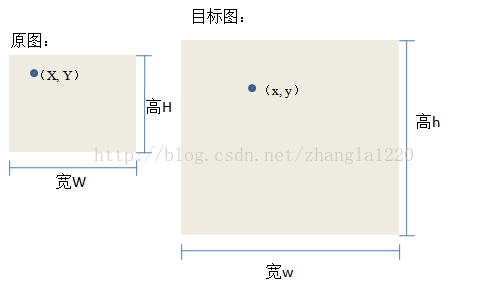
\includegraphics[width=1\linewidth]{near.jpg} 
        \end{minipage}
	\begin{minipage}[t]{0.4\linewidth}
        \centering
        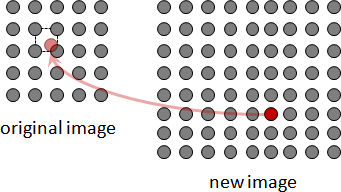
\includegraphics[width=1\linewidth]{n.png} 
        \end{minipage}
\end{frame}

\subsection*{Code}
\begin{frame}
\frametitle{Code}
\href{code/nearest.cpp}{Codes for nearest neighbor interpolation}
\end{frame}

\subsection*{Result}
\begin{frame}
\frametitle{Result}
	\begin{minipage}[t]{0.4\linewidth}
        \centering
        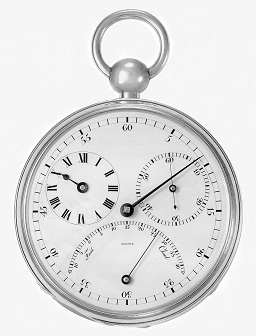
\includegraphics[width=0.5\linewidth]{1.jpg} 
        \end{minipage}
	\begin{minipage}[t]{0.4\linewidth}
        \centering
        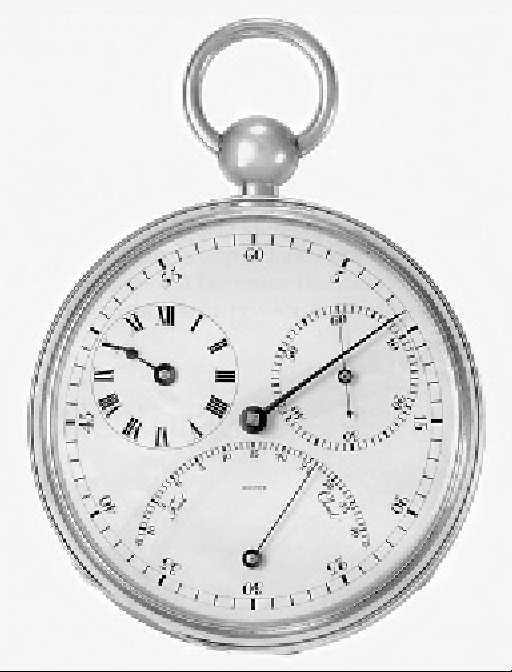
\includegraphics[width=1\linewidth]{nearest.jpg} 
        \end{minipage}

\end{frame}

\section{Bilinear interpolation}

\subsection*{Theory}
\begin{frame}
\frametitle{Bilinear interpolation}

1.$f(x,y) \approx f(0,0)(1-x)(1-y)+f(1,0)x(1-y)+f(0,1)(1-x)y+f(1,1)xy$

\mbox{}

2.
\begin{math}
v(x,y)=ax+by+cxy+d
\end{math}

\mbox{}

Coefficients:
\begin{itemize}
\item a=f(1,0)-f(0,0)
\item b=f(0,1)-f(0,0)
\item c=f(1,1)-f(0,1)-f(1,0)+f(0,0)
\item d=f(0,0)
\end{itemize}
\end{frame}

\subsection*{Code}
\begin{frame}
\frametitle{Code}
\href{code/bilinear.cpp}{Codes for bilinear interpolation}
\end{frame}

\subsection*{Result}
\begin{frame}
\frametitle{Result}
	\begin{minipage}[t]{0.4\linewidth}
        \centering
        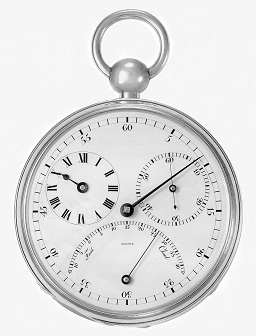
\includegraphics[width=0.5\linewidth]{1.jpg} 
        \end{minipage}
	\begin{minipage}[t]{0.4\linewidth}
        \centering
        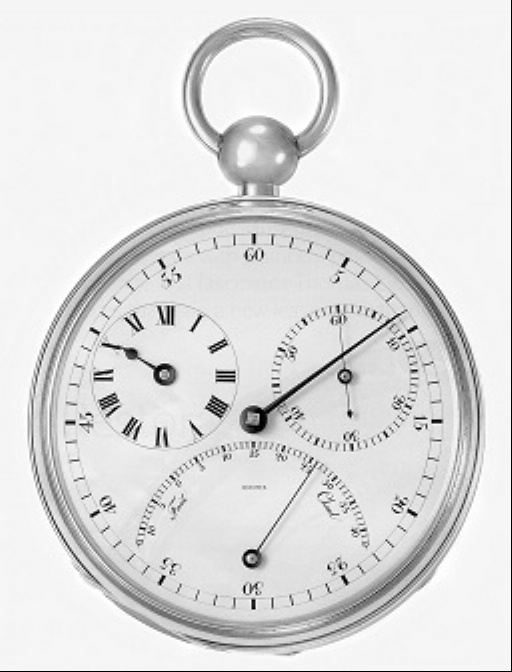
\includegraphics[width=1\linewidth]{Bilinear-pots.jpg} 
        \end{minipage}

\end{frame}
\section{Bicubic interpolation}

\subsection*{Theory}
\begin{frame}
\frametitle{Bicubic interpolation}
    	$f(x,y)=\sum _{i=0}^{3}\sum _{j=0}^{3}a_{ij}x^{i}y^{j}$

\mbox{}

The value of the coefficients $a_{ij}$ depends on the characteristic of the interpolation data.

\mbox{}

As for each dot of each unit, we have to drag the coordinates (0,0) , (1,0) , (0,1) and (1,1) into the 16 equations to get the results.
\end{frame}

\subsection*{Code}
\begin{frame}
\frametitle{Code}
\href{code/bicubic.cpp}{Codes for bicubic interpolation}

\end{frame}

\subsection*{Result}
\begin{frame}
\frametitle{Result}
	\begin{minipage}[t]{0.4\linewidth}
        \centering
        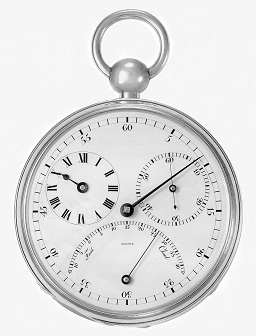
\includegraphics[width=0.5\linewidth]{1.jpg} 
        \end{minipage}
	\begin{minipage}[t]{0.4\linewidth}
        \centering
        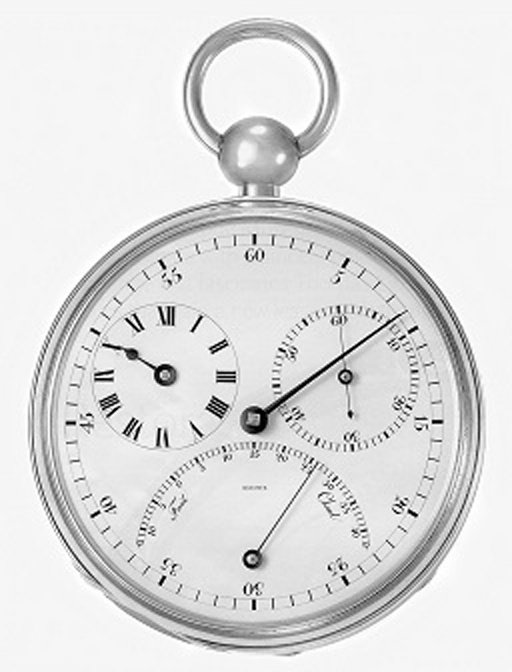
\includegraphics[width=1\linewidth]{Bicubic.jpg} 
        \end{minipage}
\end{frame}

\section{Conlusion}

\subsection{Comparison}

\begin{frame}
\frametitle{Comparison}
	\begin{minipage}[t]{0.32\linewidth}
        \centering
        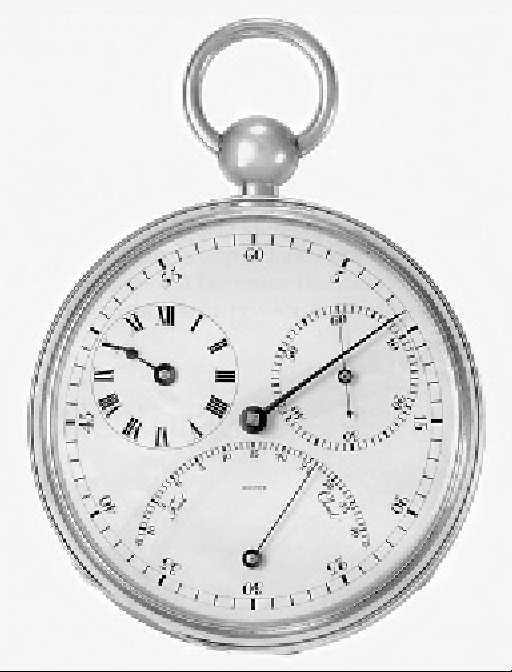
\includegraphics[width=0.9\linewidth]{nearest.jpg} 
        \end{minipage}
	\begin{minipage}[t]{0.32\linewidth}
        \centering
        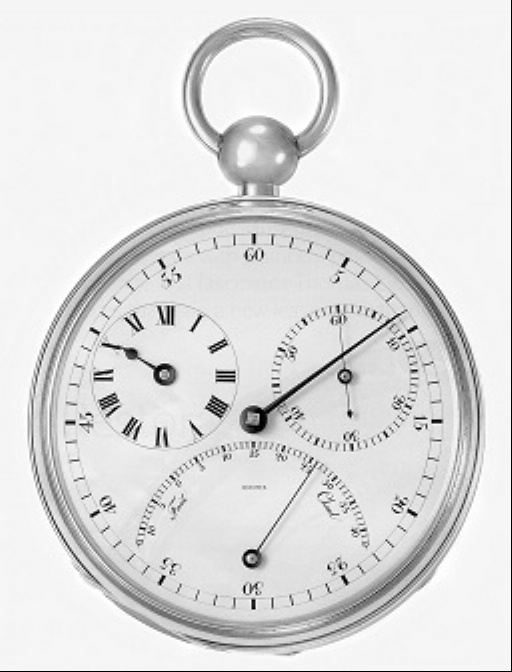
\includegraphics[width=0.9\linewidth]{Bilinear-pots.jpg} 
        \end{minipage}
	\begin{minipage}[t]{0.32\linewidth}
        \centering
        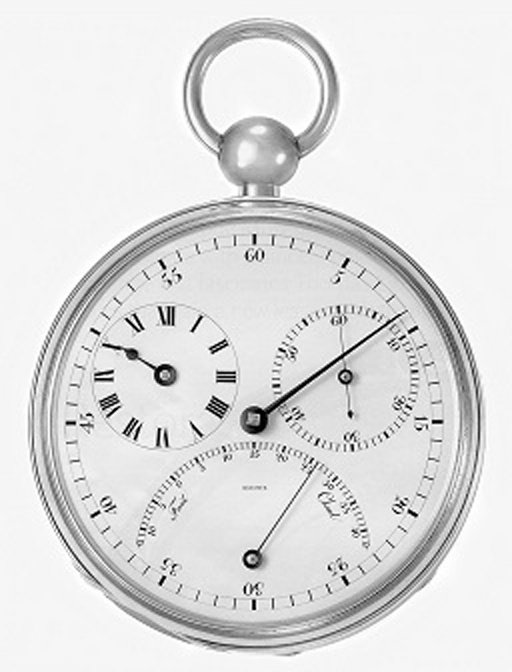
\includegraphics[width=0.9\linewidth]{Bicubic.jpg} 
        \end{minipage}
\end{frame}

\subsection{Conclusion}
\begin{frame}
\frametitle{Conclusion}
	\textbf{\color{blue}1. Completeness: }\\
	\mbox{}
	\begin{minipage}[t]{1\linewidth}
        \centering
        Bicubic interpolation  > Bilinear interpolation > Nearest neighbor interpolation
        \end{minipage}
	\mbox{}
	\begin{minipage}[t]{1\linewidth}
	\textbf{\color{blue}2. Difficulty: }\\
	\end{minipage}
	\mbox{}
	\begin{minipage}[t]{1\linewidth}
        \centering
        Bicubic interpolation  > Bilinear interpolation > Nearest neighbor interpolation
        \end{minipage}
	\mbox{}
	\begin{minipage}[t]{1\linewidth}
	\textbf{\color{red}$\rightarrow$ Bilinear interpolation satisfies the needs of most relarged images without complex arthmetic.}
	\end{minipage}
\end{frame}

\end{document}
